% !TEX TS-program = pdflatex
% !TEX encoding = UTF-8 Unicode

% This is a simple template for a LaTeX document using the "article" class.
% See "book", "report", "letter" for other types of document.

\documentclass[11pt]{article} % use larger type; default would be 10pt

\usepackage[utf8]{inputenc} % set input encoding (not needed with XeLaTeX)

%%% Examples of Article customizations
% These packages are optional, depending whether you want the features they provide.
% See the LaTeX Companion or other references for full information.

%%% PAGE DIMENSIONS
\usepackage{geometry} % to change the page dimensions
\geometry{a4paper} % or letterpaper (US) or a5paper or....
% \geometry{margin=2in} % for example, change the margins to 2 inches all round
% \geometry{landscape} % set up the page for landscape
%   read geometry.pdf for detailed page layout information

\usepackage{graphicx} % support the \includegraphics command and options

% \usepackage[parfill]{parskip} % Activate to begin paragraphs with an empty line rather than an indent

%%% PACKAGES
\usepackage{booktabs} % for much better looking tables
\usepackage{array} % for better arrays (eg matrices) in maths
\usepackage{paralist} % very flexible & customisable lists (eg. enumerate/itemize, etc.)
\usepackage{verbatim} % adds environment for commenting out blocks of text & for better verbatim
\usepackage{subfig} % make it possible to include more than one captioned figure/table in a single float
% These packages are all incorporated in the memoir class to one degree or another...

%%% HEADERS & FOOTERS
\usepackage{fancyhdr} % This should be set AFTER setting up the page geometry
\pagestyle{fancy} % options: empty , plain , fancy
\renewcommand{\headrulewidth}{0pt} % customise the layout...
\lhead{}\chead{}\rhead{}
\lfoot{}\cfoot{\thepage}\rfoot{}

%%% SECTION TITLE APPEARANCE
\usepackage{sectsty}
\allsectionsfont{\sffamily\mdseries\upshape} % (See the fntguide.pdf for font help)
% (This matches ConTeXt defaults)

%%% ToC (table of contents) APPEARANCE
\usepackage[nottoc,notlof,notlot]{tocbibind} % Put the bibliography in the ToC
\usepackage[titles,subfigure]{tocloft} % Alter the style of the Table of Contents
\renewcommand{\cftsecfont}{\rmfamily\mdseries\upshape}
\renewcommand{\cftsecpagefont}{\rmfamily\mdseries\upshape} % No bold!

%%% END Article customizations


\title{CRUD SIMPLES UTILIZANDO PYTHON E DJANGO}
\author{Antônio Fernandes De Santana Neto \\ Universidade Tiradentes}
\date{20/07/2024} 

\begin{document}


\maketitle
\begin{abstract}
Este artigo apresenta uma aplicação simples do acrônimo CRUD (Create Read Update Delete) utilizando Python como linguagem de programação e um framework seu para desenvolvimento web, Django. \\
Palavras chave: CRUD, Python, Django, Web, Aplicação. \\

This article presents a simple application of the acronym CRUD (Create Read Update Delete) using Python as a programming language and its own framework for web development, Django. \\
Keywords: CRUD, Python, Django, Web, Application.
\end{abstract}

\maketitle
\section{Introdução}
No contexto de aplicações web, manipular informações com maestria é de suma importância para o funcionamento preciso de qualquer serviço online. A um baixo nível de abstração podemos dizer que o propósito de qualquer persistencia de dados podem ser resumidas em 4 opreações: Criar, Ler, Atualizar e Deletar, respectivamente traduzidas em Create, Read, Update, Delete.\\\\
"CRUD (Criar, Ler, Atualizar, Excluir) é um acrônimo para maneiras de operar com dados armazenados. É um mnemônico para as quatro funções básicas do armazenamento persistente. [...]" (Mozila Developer Network).\\\\
Este artigo apresenta uma maneira simples de criar um CRUD em poucos minutos utilizando a linguagem de programação Python e uma coleção de ferramentas prontas (Framework) para o desenvolvimento web, Django.

\maketitle
\section{Utilidades}
A aplicação desenvolvida pode ser usada para maior parte dos cenários, portanto que haja seus respectivas mudanças relacionadas a sua regra de negócio. Com um serviço versátil e facilmente auditável pelo painel admnistrativo nativo, torna as possíbilidades mais variadas e aplícaveis dentro do seu determinado contexto.

\maketitle
\section{Metodologia}
Será abordado um gerenciamento de usuários, contendo todas as operações do acrônimo CRUD de forma visual, intuitiva e de fácil compreensão. Será criado um "super usuário" que terá a autonômia máxima no sistema, pondendo inclusive gerenciar os outros usuários já presentes.\\\\
Uma possibilidade de extensão que estará disponível, todavia não abordado nesse artigo, é a criação de "grupos de usuários", onde é possivel auditar as permissões de todos os outros usuários.

\maketitle
\section{Materiais e Métodos}
\subsection{Sistema Operacional}
Neste artigo foi utilizado o sistema operacional Linux (Linux debian 5.10.0-18-amd64 1 SMP Debian 5.10.140-1 (2022-09-02) x86-64). \\Mais informações em: https://packages.qa.debian.org/l/linux.html 
\subsection{Python 3.11.9}
Foi utilizado a linguagem de programação Python em sua versão 3.11.9.\\ Para mais informações: https://www.python.org/downloads/release/python-3119/

\maketitle
\section{Implementação}
\subsection{Criaçao do diretório}
Para fins de organização, foi criado uma pasta chamada "crud" e posteriormente adentrado na mesma, como ilustra a imagem a seguir:\\
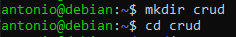
\includegraphics[]{C:/Users/Antônio/Downloads/s1.PNG}
\subsection{Ambiente Virtual}
Também para fins de organização, será criado um ambiente virtual onde instalaremos o Django e todas suas respectivas dependências.\\
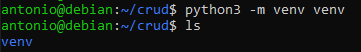
\includegraphics[]{C:/Users/Antônio/Downloads/s2.PNG}\\
Depois de criar o ambiente virtual, iremos ativar o mesmo:\\
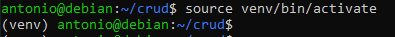
\includegraphics[]{C:/Users/Antônio/Downloads/s3.PNG}
\subsection{Django}
\subsubsection{Instalação}
Após configurar e acessar o ambiente virtual, instala-se o Django\\
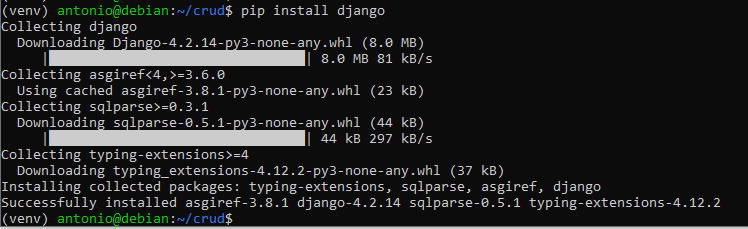
\includegraphics[width=150mm,scale=1]{C:/Users/Antônio/Downloads/s4.PNG}
\subsubsection{Criação da aplicação}
Agora com o Django instalado, basta criar o projeto:\\
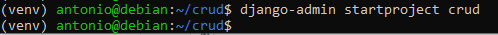
\includegraphics[]{C:/Users/Antônio/Downloads/s5.PNG}
\subsubsection{Migrations}
Com a aplicação já criada, precisamos modelar o banco de dados que armazenará as informações. O Django já traz um recurso para facilitar todo o processo de modelagem, chamado de "Migrations", que basicamente são arquivos estáticos que conseguem salvar os processos de alterações nas tabelas cronologicamente. "Migrations são a maneira do Django de propagar as alterações feitas em seus Models (adicionando um campo, excluindo um modelo, etc.) em seu esquema de banco de dados." (Documentação oficial do Django). Estes "Models" são arquivos criados manualmente pelo desenvolvedor para modular alguma tabela do banco de dados, todavia existem algumas que já vem por padrão criadas, dentre elas, o Model de "User" (usuário). Então podemos aplicar os arquivos de migrations que já vem com o framework e teremos o banco de dados modularizados para auditar usuários.\\
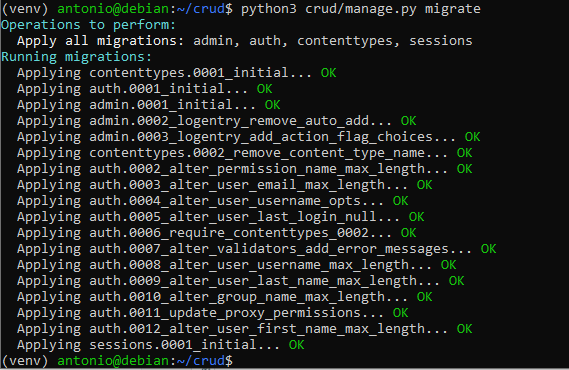
\includegraphics[]{C:/Users/Antônio/Downloads/s6.PNG}
\subsubsection{Super Usuário}
Quando todas as aplicações dos arquivos de Migrations forem aplicados, poderemos criar o "super usuário" que auditará toda e qualquer informação do sistema. Neste caso foi criado com o nome de usuário "root" e senha "root".\\
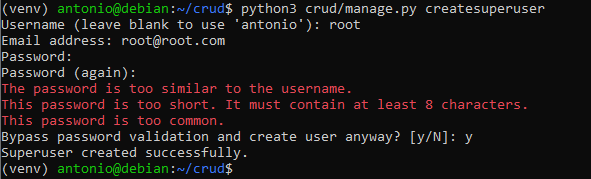
\includegraphics[]{C:/Users/Antônio/Downloads/s7.PNG}
\subsubsection{Executar a Aplicação}
Depois de seguir todos os passos anteriores, a aplicação está pronta para ser utilizada. Após executada, estará disponível em seu endereço local na porta 8000 por padrão.\\
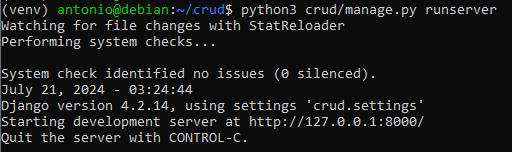
\includegraphics[]{C:/Users/Antônio/Downloads/s8.PNG}

\maketitle
\section{Utilizando a Aplicação}
Após completar todo o processo de implementação, a aplicação deve estar disponível em "http://localhost:8000". Acessando o endereço indicado este é o resultado:\\
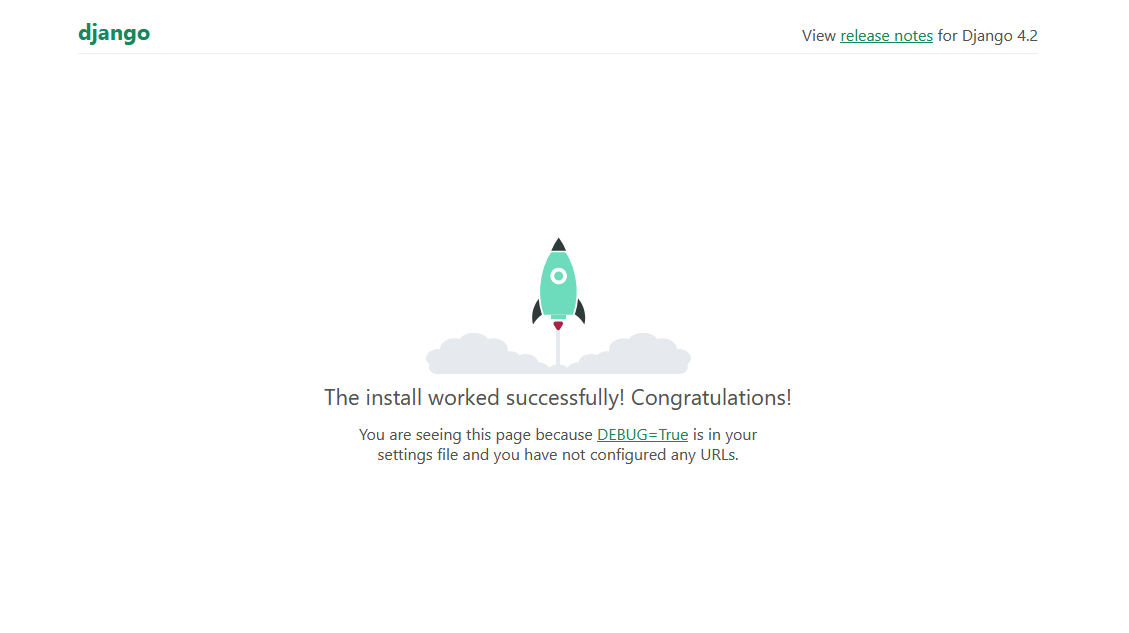
\includegraphics[width=150mm,scale=0.7]{C:/Users/Antônio/Downloads/s9.png}\\
Acessando a rota "/admin" temos o seguinte resultado:\\
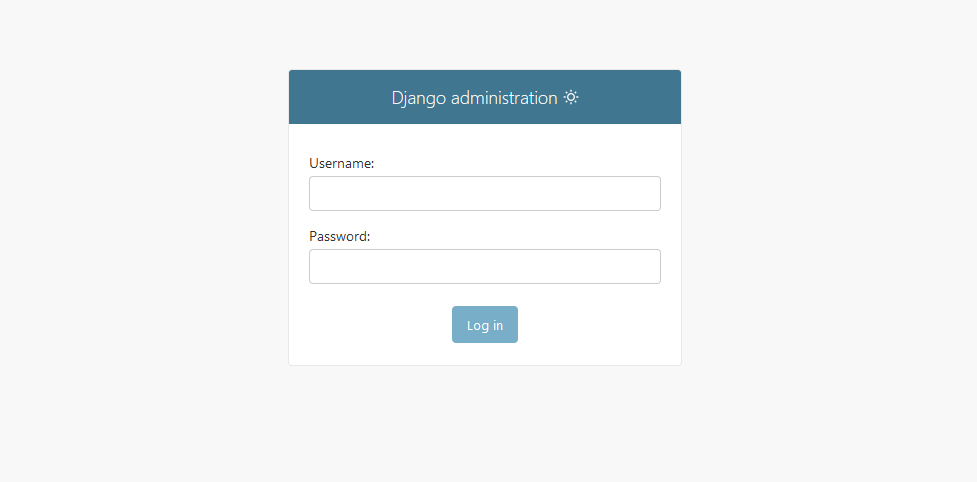
\includegraphics[width=150mm,scale=0.7]{C:/Users/Antônio/Downloads/s10.PNG}\\
Utilizando o acesso anteriormente criado para o super usuario, é possivel efetuar o login e acessar o ambiente admnistrativo.\\
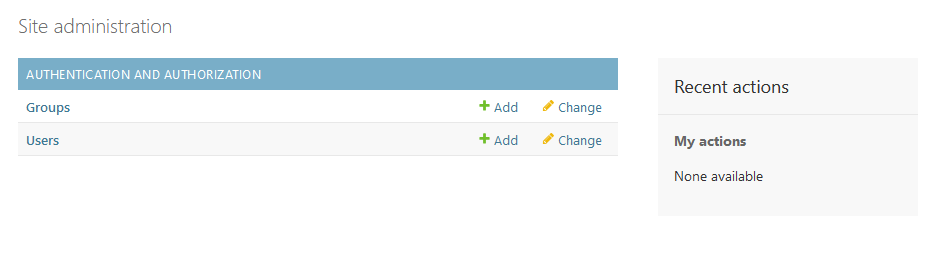
\includegraphics[width=150mm,scale=0.7]{C:/Users/Antônio/Downloads/s11.PNG}

\maketitle
\section{Resultados}
Os resultados incluem um aplicativo web funcional que permite  realizar operações de criação, leitura, atualização e exclusão de usuários.

\maketitle
\section{Conclusão}
Em conclusão, este artigo demonstrou a viabilidade e a simplicidade de implementar persistência de dados utilizando Python e Django. A abordagem passo a passo proporcionou uma compreensão clara das etapas necessárias para construir uma aplicação web básica.\\\\
A implementação de CRUD é fundamental em praticamente qualquer aplicação web, e dominar essa habilidade com Django permite a criação de soluções eficientes e escaláveis.


\end{document}
